\subsection{First Isomorphism Theorem}
\begin{frame}
	\frametitle{First Isomorphism Theorem}
	\begin{theorem}
		Let $\phi : G \to G'$ be a group homomorphism with kernel $K$.
		And let $\gamma_K : G \to G/K$ be the canonical homomorphism.
		Then there is a unique isomorphism $\mu : G/K \to \phi[G]$
		such that $\phi(x) = \mu(\gamma_K(x))$.
	\end{theorem}
	\begin{figure}
	\centering
	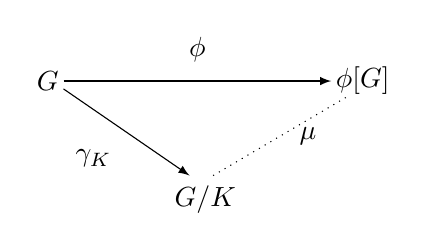
\begin{tikzpicture}
		\draw (0,1.5) node {$G$};
		\draw (2,0) node {$G/K$};
		\draw (4,1.5) node {$\phi[G]$};
		\draw[-latex] (0.2,1.4) -- node(e1)[sloped,label=below:$\gamma_K$]{} (1.8,0.3);
		\draw[-latex] (0.2,1.5) -- node(e2)[label=above:$\phi$]{} (3.6,1.5);
		\draw[dotted] (2.1,0.3) -- node(e2)[label=right:$\mu$]{} (3.8,1.3);
	\end{tikzpicture}
	\caption{First Isomorphism Theorem}
\end{figure}
\end{frame}

\begin{frame}
	\frametitle{First Isomorphism Theorem}
	\setbeamercovered{transparent}
	Let $G,G'$ be groups. And $\phi : G \to G'$ be a group homomorphism.
	\uncover<2-3>{Let $g \in G$.}
	\uncover<3>{Let $K = \ker(\phi)$.\\ That is, $\phi[K] = e'$ or $\forall k \in K,\ \phi(k) = e'$.\\ Then $\phi[gK] = \phi(g)$, since $\phi(gk)=\phi(g)\phi(k) = \phi(g)$.}

	\uncover<4>{Let $\gamma_K : G \to G/K$ be a canonical homomorphism.\\ Then $\mu : G/K \to \phi[G]$ defined by $\mu(gK) = \phi(g)$ is an isomorphism.}

	\begin{figure}
	\centering
	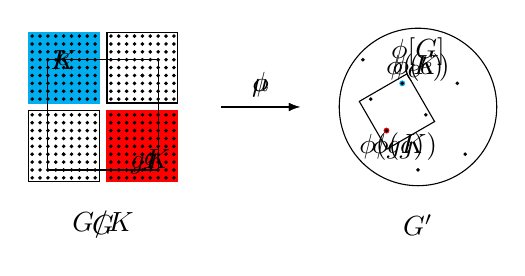
\begin{tikzpicture}
		%\draw[cyan,fill = cyan] (2.05,1.05) rectangle (2.95,1.95);
		\draw<1-2>[cyan,fill = cyan] (0.5,1.4) circle[radius=0.03]; %e
		\draw<4>[cyan,fill = cyan] (0.5,1.4) circle[radius=0.03]; %K
		\draw<4>[red,fill= red] (1.5,0.4) circle[radius=0.03]; %gK
		\draw<2-3>[red,fill = red] (1.6,0.5) circle[radius=0.03]; %g
		\draw<2->[cyan,fill = cyan] (4.8,1.3) circle[radius = 0.03]; %\phi(e)
		\draw<2->[red,fill = red] (4.6,0.7) circle[radius = 0.03]; %\phi(g)

		\draw<1-3>[-latex] (2.5,1) -- node[above]{$\phi$} (3.5,1); 
		\draw<4>[-latex] (2.5,1) -- node[above]{$\mu$} (3.5,1); 

		%Group G
		%coset division G/K
		\draw<3> (0.05,0.05) rectangle (0.95,0.95);
		\draw<3>[cyan,fill = cyan] (0.05,1.05) rectangle (0.95,1.95);
		\draw<3>[red,fill= red ] (1.05,0.05) rectangle (1.95,0.95);
		\draw<3> (1.05,1.05) rectangle (1.95,1.95);
		%elements of G
		\foreach \ii in {0,1}{
			\foreach \jj in {0,1}{
				\foreach \kk in {1,...,9}{
					\foreach \ll in {1,...,9}{
						\draw<1-3>[black,fill=black] (\ii.\kk,\jj.\ll) circle[radius=0.015];
			}}}}
		%elements of G/K
		\draw<4>[black,fill=black] (0.5,0.4) circle[radius=0.015];
		\draw<4>[black,fill=black] (0.5,1.4) circle[radius=0.015];
		\draw<4>[black,fill=black] (1.5,0.4) circle[radius=0.015];
		\draw<4>[black,fill=black] (1.5,1.4) circle[radius=0.015];
		%Group G'
		\draw (5,1) circle[radius = 1cm];
		%elements of G'
		\draw (4.8,1.3) circle[radius = 0.015];
		\draw (4.6,0.7) circle[radius = 0.015];
		\draw (5.1,0.9) circle[radius = 0.015];
		\draw (4.4,1.1) circle[radius = 0.015];
		\draw (4.3,1.6) circle[radius = 0.015];
		\draw (5.6,0.4) circle[radius = 0.015];
		\draw (5,0.2) circle[radius = 0.015];
		\draw (5.5,1.3) circle[radius = 0.015];

		\draw<4>[rotate=30,shift={(4.22,-1.9)}] (0,0) rectangle (0.7,0.7);
		\draw<4> (0.3,0.2) rectangle (1.7,1.6);

		\draw<1-3> node at (1,-0.5) {$G$};
		\draw<4> node at (1,-0.5) {$G/K$};
		\draw node at (5,-0.5) {$G'$};
		\draw<1-2> node at (0.5,1.6) {$e$};
		\draw<3-3> node at (0.5,1.6) {$K$};
		\draw<2> node at (1.6,0.3) {$g$};
		\draw<3> node at (1.6,0.3) {$gK$};
		\draw<1> node at (5.0,1.5) {$e'$};
		\draw<2> node at (5.0,1.5) {$\phi(e)$};
		\draw<3> node at (5.0,1.5) {$\phi(K)$};
		\draw<2> node at (4.75,0.5) {$\phi(g)$};
		\draw<3> node at (4.75,0.5) {$\phi(gK)$};
		\draw<4> node at (5,1.7) {$\phi[G]$};
	\end{tikzpicture}
	\end{figure}
\end{frame}
